
\section{Introduction}
	\IEEEPARstart{T}{he} aim of this project was to investigate how the diversity of an genetic algorithm's population effects the performance of Multi-Layer Perception Neural Network trained by said algorithm. 
	A substantial amount of research has already been conducted into how the effectiveness of Hyper-heuristic's can be improved by encouraging diversity in the individual sub-heuristics - this investigation was designed to asses if a similar approach to Hyper-heuristic diversity could be applied to an genetic algorithm to improve it's fitness
	
\section{Approach}
	Investigation was conducted by exploring how different types of Parent Selection, Child Crossover, Mutation, and Immigrant Injection can alter the overall diversity of an genetic algorithm's population - and how in turn that effects the overall fitness of the algorithm.
	
	\subsection{Background}
		Stuff about hyper-heuristics goes here. Get those references, son.
		\cite{Hong16112004} \cite{hart2017constructing}
	
	\subsection{Algorithm Design}
		A simple genetic algorithm of similar style to supplied version was used throughout this investigation. Unless otherwise stated, a single generation of the algorithm was as follows:

		\begin{algorithm}[H]
			\caption{Genetic Algorithm Pseudocode}
			A random population is generated\\
			Two individuals are selected from the population as parents\\
			Two children are generated from  the parents\\
			The children are mutated\\
			Children replace two worst individuals in the population
		\end{algorithm}
		
		Upon completion, the fittest chromosome produced by the algorithm were used as the weights for a multi-layer perception neural network, which attempted to perform a function estimation using pre-supplied training data. Once that algorithm was run for a predetermined number of generations, a final test using a separate set of data was used to determine the overall effectiveness of the neural network, and in thus, the effectiveness of the genetic algorithm. Details of selection, crossover and mutation methods are presented below.  
			
	\subsection{Algorithm Operators}
		\subsubsection{Selection}
			While the provided \texttt{selectRandom} function was a perfectly valid solution to increasing the diversity of selected parents - alternative selection functions had to be designed to allow for comparison.
			
			\texttt{selectRandom}: The provided selection method operates by simply choosing two random individuals from the population. This selection function should be considered the most diverse, as every individual in the population has an equal chance of being selected to become a parent - regardless of their fitness
	
			\texttt{selectElite}: This selection method operates by choosing the two individuals with the best and second-best fitness. From a ignorant approach, this may seem to be a valid section tactic, in reality however this method is likely to cause the population to reach a local maxima within a relatively small number of generations. \texttt{selectElite} was included in this investigation to provide evidence that a lack of diversity in the population may be deferential to its potential fitness.
			
			\texttt{selectTournament}: This function was designed to randomly choose a designated number of individuals - and the individual in the group with the best fitness goes forward as a parent. The number of individuals in the tournament directly alters the selection pressure - lager tournaments have a smaller chance of a weaker individual being chosen for crossover. This selection method should prove adequate in diversifying the population - however it is unlikely to be as pronounced as the \texttt{selectRandom} function.
			
			\texttt{selectRoulette}: A roulette selection has to potential to pick any individual in the population, proportional to its fitness - e.g. an individual with a fitnesses of 10 is twice as likely to be picked over an individual with a fitness of 5. While individuals with high fitness are more likely to be selected by this function, it is not guaranteed - ensuring this function is suitable for the diversification of the population.
		
		\subsubsection{Crossover}
			All  crossover methods utilised in this project produced a pair children which were then introduced to the algorithm population by replacing the to two individuals with the worst fitness. Crossover is the most typical way to add diversity to an genetic algorithm, however the children's similarity to their parent's is determined by the type of cross over used.
			
			\begin{figure*}[]
				\centering
				\subfloat[Single point crossover]{
					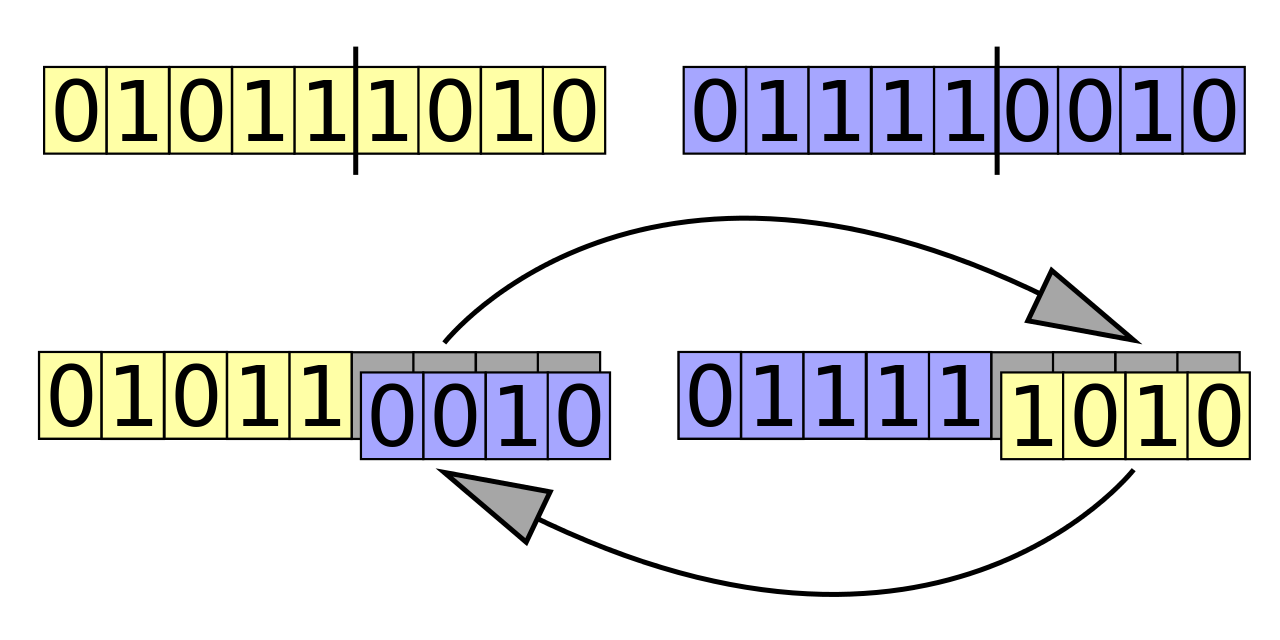
\includegraphics[width=2.5in]{crossover_single}%
					\label{fig_cross_single}
				}
				\hfil
				\subfloat[Double point crossover]{
					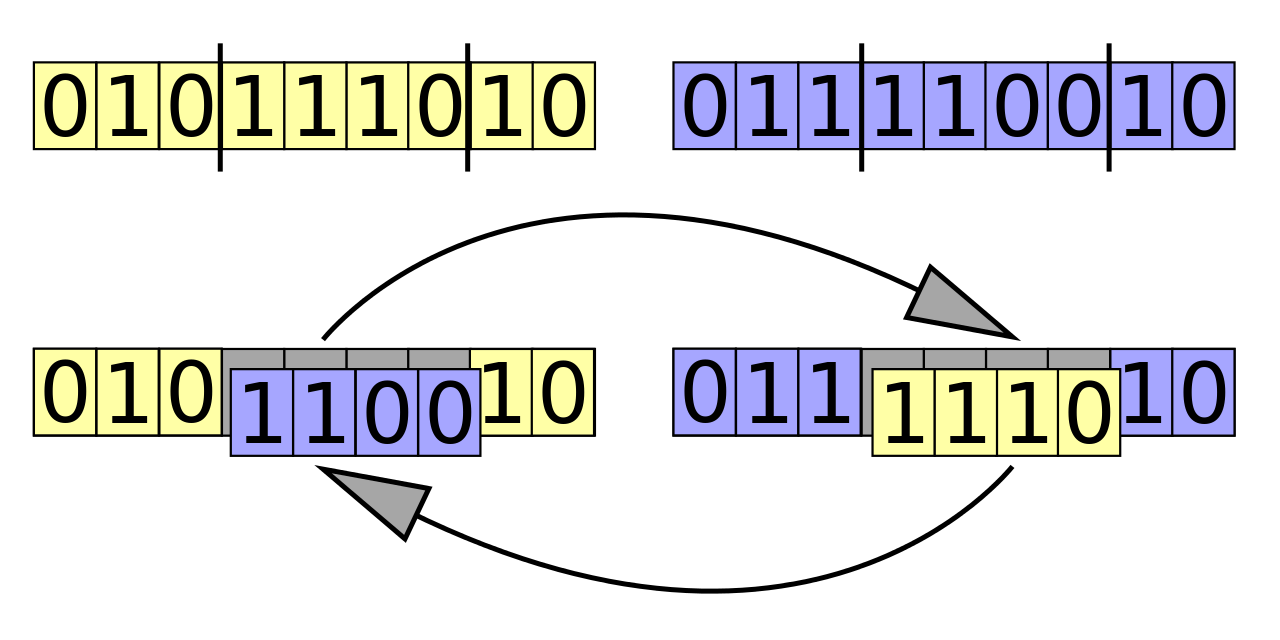
\includegraphics[width=2.5in]{crossover_double}%
					\label{fig_cross_double}
				}
				\newline
				\subfloat[Uniform crossover]{
					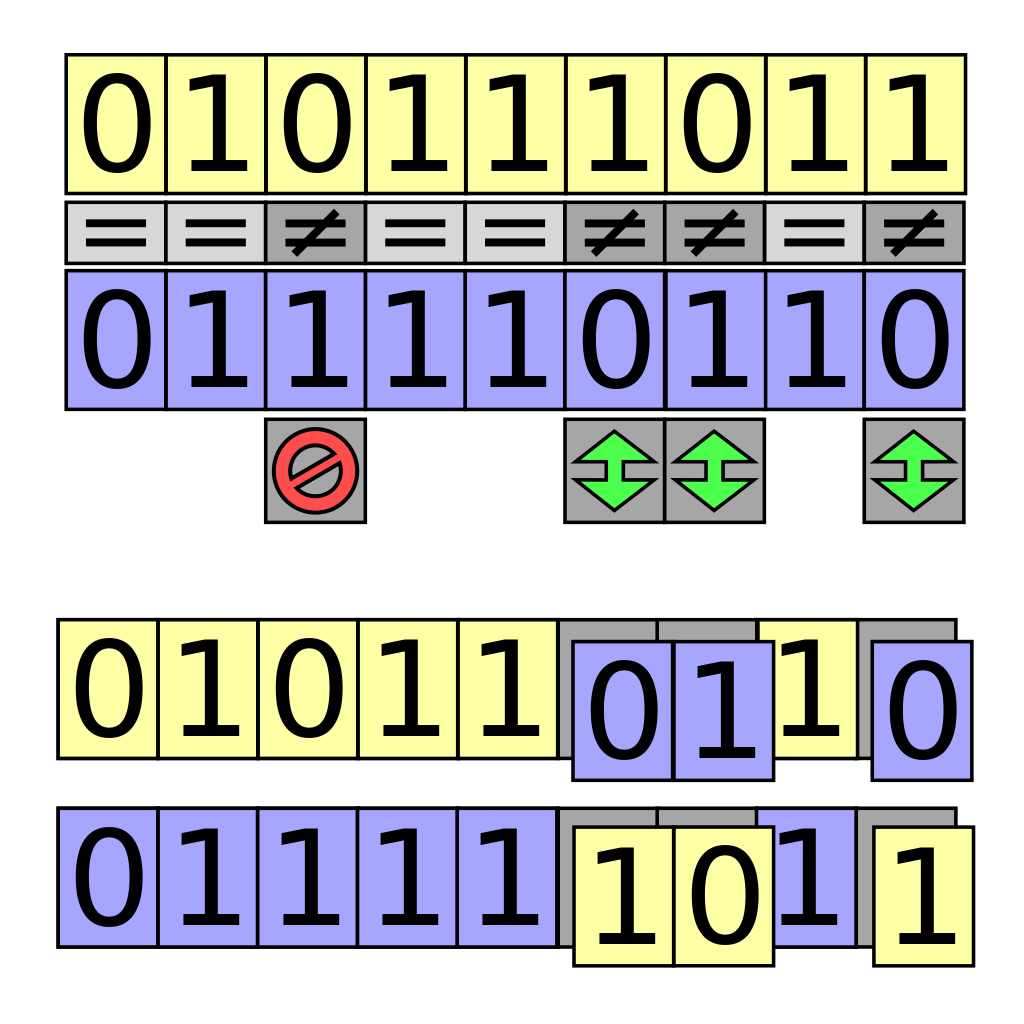
\includegraphics[width=1.25
					in]{crossover_uniform}%
					\label{fig_cross_uni}
				}
				\caption{Examples of three types of crossover function.}
				\label{fig_cross}
			\end{figure*}
	
			\texttt{crossoverClone}: The provided crossover function produces a pair of children, each identical to one of the parents. The use of this kind crossover will result in the eventual homogenization of the algorithm's population - significantly reducing the diversity of the chromosomes. 
		
			\texttt{crossoverSingle}: A single-point crossover method uses a random number to determine a crossover point in two newly created children chromosomes. Each child is then given a number of genes from one parent, up to the crossover point, when they then receive genes from the other parent. This crossover method produces 2 inversely mirrored children - in extreme cases can produce two children identical to the parents, reducing the overall diversity of the population by introducing duplicates. 
			
			\texttt{crossoverDouble}: Extremely similar to the  \texttt{crossoverSingle} function, with the caveat being that two crossover points are generated. With the addition of a second pivot point on which to swap which parent is passing genes, the chances of producing children similar to the parents is reduced - assuming that the two parents are not already similar in terms of genes.
			
			\texttt{crossoverUniform}: Unlike the previous segment based crossovers, a uniform crossover function operates on a gene level. Each gene in a child is copied from one of the two parents depending on the value of a randomly generated number e.g. on the value of 0 the first parent's gene is used, on the value of 1 the second parent's gene is copied. Like the other crossover functions, \texttt{crossoverUniform} produces a set of mirrored children. This cross over method has the potential to produce the most diverse children from a set of parents. 
			
		\subsubsection{Mutation}
			Mutation of chromosomes is yet another area of a genetic algorithm were diversity can be introduced. No form of mutation was provided, so a simple boundary mutation function was designed within the algorithm presented, mutation was only applied to child chromosomes produced by a cross over function.
			
			\texttt{mutateBoundary}: This mutation function operates over every gene in a chromosome, producing a random \texttt{double} between 0 and 1 for each one, if the double is less than a predetermined value (\texttt{mutateRate}) then the current gene is altered by adding  or subtracting a second predetermined value (\texttt{mutateChange}) to the gene. Once all the genes in a chromosome were been considered for mutation any genes that were pushed outside their maximum or minimum boundary are then brought back in line.
		
	\subsection{Neural Network}
		As the primary goal of this report was to investigate how the diversity of the genetic algorithm's population changed its effectiveness, very few of the Neural network's parameters were changed or investigated.
		
		\texttt{geneMax} \& \texttt{geneMin}: The values of 5.0 and -5.0 were used respectively for the maxim and minimum possible values of gene for each chromosome. While the systematic altering and testing of these values could have led to a super solution - leaving them at the default values ensured the other test could be compared fairly.
		
		\texttt{hiddenNodes}: The number of nodes in the hidden layer was the one neural network parameter that was changed from the default. Preliminary testing indicated that when approximating functions A and B 5 hidden nodes produced the best result. When approximating function C however, 2 hidden nodes proved to be the most effective. These values were used in all future tests to ensure consistent and fair comparison. 
		
\section{Experiments \& Analysis}
	What I did

\section{Results}
	What I found

\section{Conclusion}
	Summary

\section{Future Work}
	What to do in the future
	